\chapter{Tensor networks}
\label{ch:tn}

Quantum many-body systems are naturally represented in spaces of high-rank tensors, and the demand to decompose them into smaller tensors has arisen in studies of their entanglement properties~\cite{white1992density}. The diagrammatic notations of tensors, namely Penrose graphical notations~\cite{penrose1971applications}, have greatly eased the construction and reasoning of complicated contractions with multiple tensors, known as tensor networks~\cite{bridgeman2017hand, orus2014practical}. Their use has been widely promoted in various fields of physics beyond condensed matters, including quantum computing~\cite{feynman1986quantum, nielsen2010quantum}, high-energy physics~\cite{banuls2018tensor, banuls2020review}, and quantum gravity~\cite{perez2013spin, you2016entanglement, hayden2016holographic, asaduzzaman2020tensor}.

Tensor networks can also be used as variational ansatzes, which enable exact and efficient summation over exponentially many configurations, instead of Monte Carlo sampling. Compared to neural networks, tensor networks are usually more controllable and systematically improvable, in the sense that they have few hyperparameters prone to manual tuning, and by tuning these hyperparameters, we can continuously improve the accuracy of variational approximation at the cost of more computation.

\section{Tensor diagram notations}

\begin{figure}[htb]
\centering
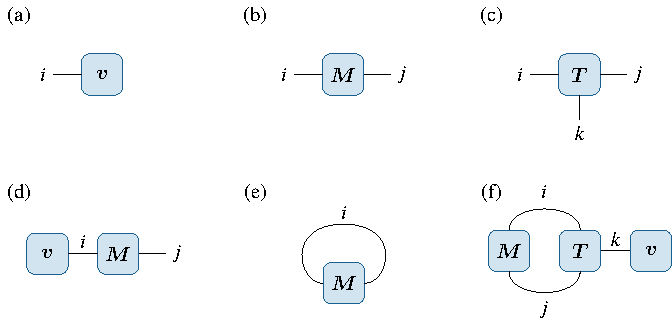
\includegraphics[width=0.7\linewidth]{ch8/tensors.pdf}
\caption[Tensor diagram notations]{
Examples of tensor diagram notations.
(a) A vector $\bm{v}$ with an index $i$.
(b) A matrix $\bm{M}$ with two indices $i, j$.
(c) A tensor $\bm{T}$ with three indices $i, j, k$.
(d) The matrix-vector multiplication $\sum_i v_i M_{i j}$, where $j$ is left as a free index.
(e) The matrix trace $\sum_i M_{i i}$.
(f) The tensor contraction $\sum_{i, j, k} T_{i j k} M_{i j} v_k$.
}
\label{fig:tensors}
\end{figure}

For the purpose of this thesis, we view tensors as multidimensional arrays, and we do not emphasize their invariance under symmetry operations. In the diagrammatic notations, each tensor is a node in the diagram, and its indices are denoted by ``legs'' stretching out from the node\footnote{Some literature distinguishes between covariant and contravariant indices, but we do not  distinguish between them in this thesis, and we allow contracting any two indices as long as they are defined in the same space.}. The contraction between two indices is denoted by connecting the two legs. Some examples of tensor diagrams are shown in \cref{fig:tensors}.

In principle, when the tensor is not symmetric in any two indices, we need to specify which leg corresponds to which index, e.g., whether \cref{fig:tensors}~(f) represents $\sum_{i, j, k} T_{i j k} M_{i j} v_k$ or $\sum_{i, j, k} T_{i j k} M_{j i} v_k$. But we usually omit this specification for brevity when it can be inferred from the context. Also, we omit the names of indices when not needed.

\section{Matrix product state (MPS)}

\begin{figure}[htb]
\centering
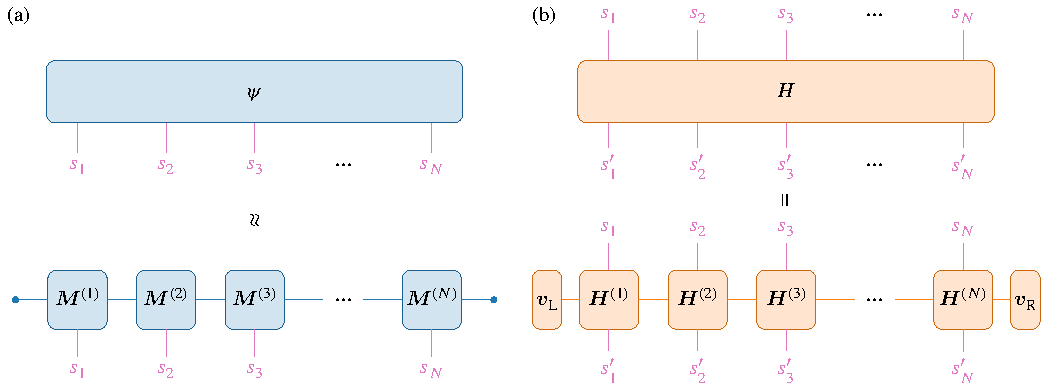
\includegraphics[width=\linewidth]{ch8/mps_mpo.pdf}
\caption[Matrix product state (MPS) and matrix product operator (MPO)]{
(a) A quantum many-body wave function $\psi(s_1, \ldots, s_N)$ approximated by a matrix product state (MPS).
(b) A Hamiltonian $H(s_1, \ldots, s_N; s'_1, \ldots, s'_N)$ represented by a matrix product operator (MPO).
The pink legs can take spin values, the blue legs have the MPS bond dimension $\chi$, the orange legs have the MPO bond dimension $\chi_H$, and the solid dot denotes summing over an index.
}
\label{fig:mps-mpo}
\end{figure}

\begin{figure}[htb]
\centering
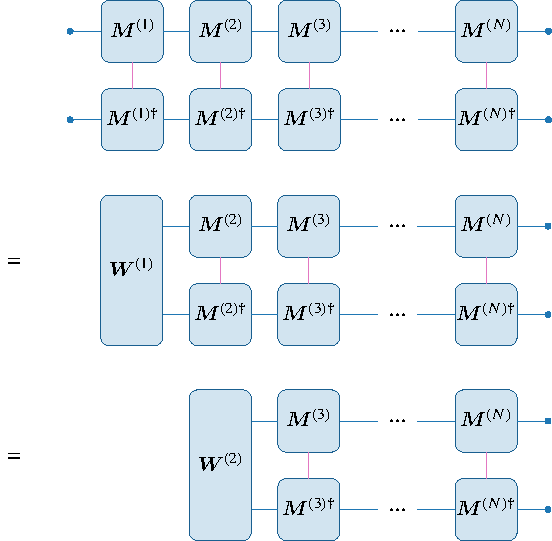
\includegraphics[width=0.6\linewidth]{ch8/mps_contract.pdf} \hspace{2cm}
\caption[Sequential contraction of MPS]{
Sequential contraction of an MPS and its conjugate, where $\mW^{(i)}$ is the intermediate result after the $i$-th step. In each step, we contract $\mW^{(i - 1)}$ and $\mM^{(i)}$, then contract the result with $\mM^{(i) \dagger}$ to obtain $\mW^{(i)}$, which takes $O(\chi^3)$ time and $O(\chi^2)$ space.
}
\label{fig:mps-contract}
\end{figure}

Ancestral sampling~\cite{wei2022sequential}

\section{Density matrix renormalization group (DMRG)}

\begin{figure}[htb]
\centering
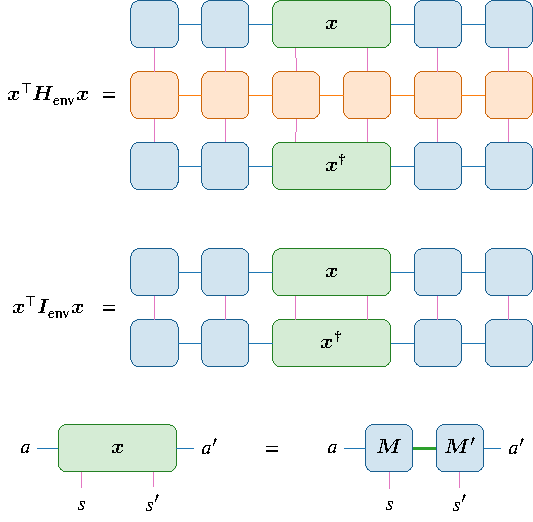
\includegraphics[width=0.7\linewidth]{ch8/dmrg.pdf}
\caption[Density matrix renormalization group (DMRG)]{
Density matrix renormalization group (DMRG)
}
\label{fig:dmrg}
\end{figure}

\section{Tensor networks with higher-dimensional geometries}

\begin{figure}[htb]
\centering
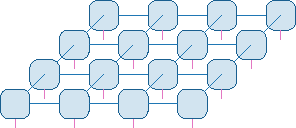
\includegraphics[width=0.5\linewidth]{ch8/peps.pdf}
\caption[Projected entangled pair states (PEPS)]{
Projected entangled pair states (PEPS)
}
\label{fig:peps}
\end{figure}

\chapter{Tensor-RNN: bridge between tensor networks and neural networks}

Another architecture~\cite{hibat2021variational, hibat2022supplementing}

Mixture of neural and tensorial layers~\cite{chen2023antn}

Recurrent arithmetic circuits~\cite{levine2017long, levine2019quantum}

\chapter{VarBench: variational benchmarks for quantum many-body systems}
\label{ch:varbench}
